%*----------- SLIDE ------------------------------------------------------------
\begin{frame}
    %\transdissolve[duration=0.5]
    %\hspace*{-1cm}
    \begin{columns}
        %\column{.01\textwidth}
        \column{0.30\textwidth}
        ~\hfill
            \begin{beamercolorbox}[sep=8em, colsep*=18pt, wd=\textwidth,ht=\paperheight]{title page header}
                \begin{center}
                    \textbf{\huge{Introdução}}\par
                    \vspace*{0.3cm}
                    % \textbf{\huge{LIBERDADE}}\par
                    \vspace*{0.3cm}
                    The Stanford Cart and The CMU Rover
                \end{center}
            \end{beamercolorbox}%         
        \column{.05\textwidth} 
        \column{.65\textwidth}
        \begin{center}
            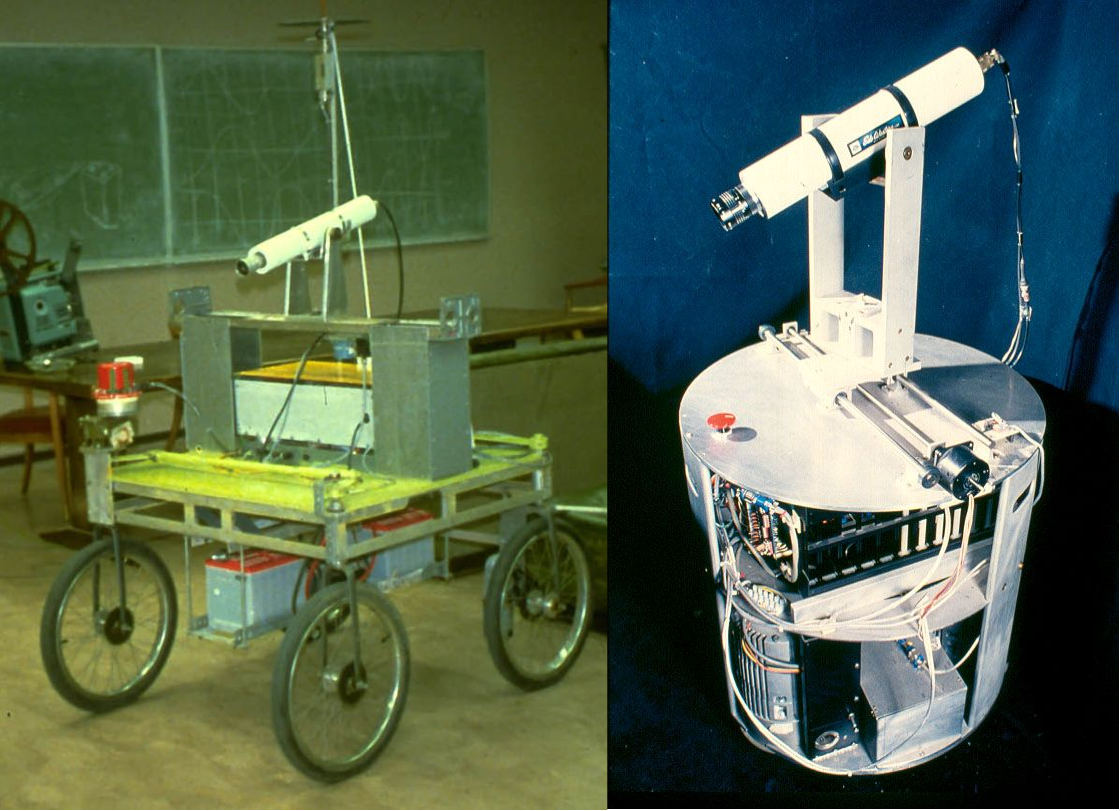
\includegraphics[width=\textwidth]{TheStanfordCart/intro.png}
        \end{center}
            
    \end{columns}
  
%*----------- notes
    \note[item]{Notes can help you to remember important information. Turn on the notes option.}
 \end{frame}
%-
%*----------- SLIDE -------------------------------------------------------------
\begin{frame}[t]{The Stanford Cart}
    \begin{columns}
        \column{.05\textwidth}
        \column{.45\textwidth}
            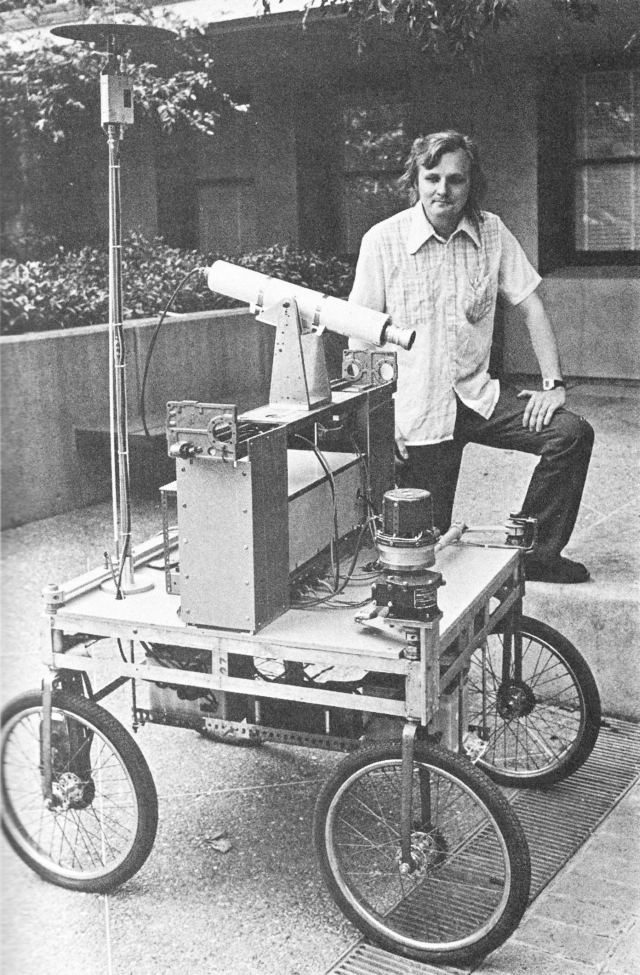
\includegraphics[width=0.6\textwidth, clip, trim = 0 0 0 0]{TheStanfordCart/StanfordCart-Moravec-x640.jpg}
        \column{.5\textwidth}
            % \centering
            Robô móvel equipado com uma câmera de TV
            \begin{itemize} 
                \item Desenvolvido por Hans. P. Moravec
                \item Utiliza visão stereo
                \item Utilizado em pesquisas de navegação visual
            \end{itemize}
            \end{columns}
%*----------- notes
    \note[item]{Notes can help you to remember important information. Turn on the notes option.}
\end{frame}

%*----------- SLIDE -------------------------------------------------------------
\begin{frame}[t]{ Hans P. Moravec}
    \begin{columns}
        \column{.05\textwidth}
        \column{.50\textwidth}
        \begin{itemize} 
            \item Nascido em 30 de novembro de 1948
            \item Realizou pesquisas nas universidades de Stanford e Carnegie Mellon
            \item Principais áreas: Robótica e inteligência artificial
        \end{itemize}
        \column{.45\textwidth}
            \centering
            \vspace*{0.8cm}
            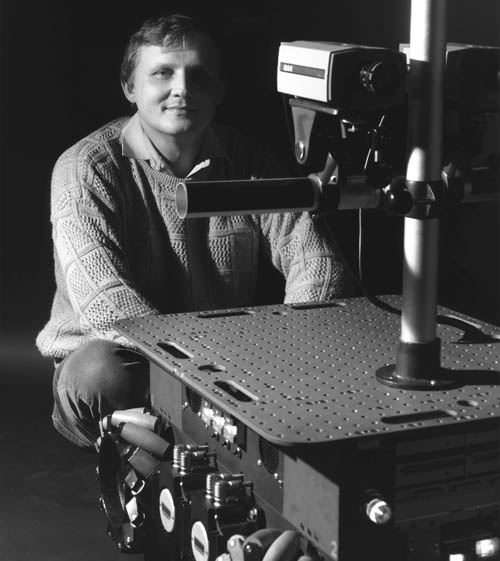
\includegraphics[width=0.8\textwidth, clip, trim = 0 0 0 0]{TheStanfordCart/moravec.jpg}
        \end{columns}
%*----------- notes
    \note[item]{Notes can help you to remember important information. Turn on the notes option.}
\end{frame}

%*----------- SLIDE -------------------------------------------------------------
\begin{frame}[t]{The Stanford Cart}
    \framesubtitle{Rotinas}
    \begin{columns}
        \column{.01\textwidth}
        \column{.49\textwidth}
        O robô obtêm 9 fotos através de sua câmera, e a partir destas imagens é capaz de
        deduzir a transformada da sua coordenada 3D e a posição 3D dos features das imagens
        \vspace*{0.8cm}
        
\includegraphics[width=\textwidth, clip, trim = 0 0 0 0]{TheStanfordCart/diagram.png}
        \vspace*{0.3cm}
        \column{.5\textwidth}
        % \centering
            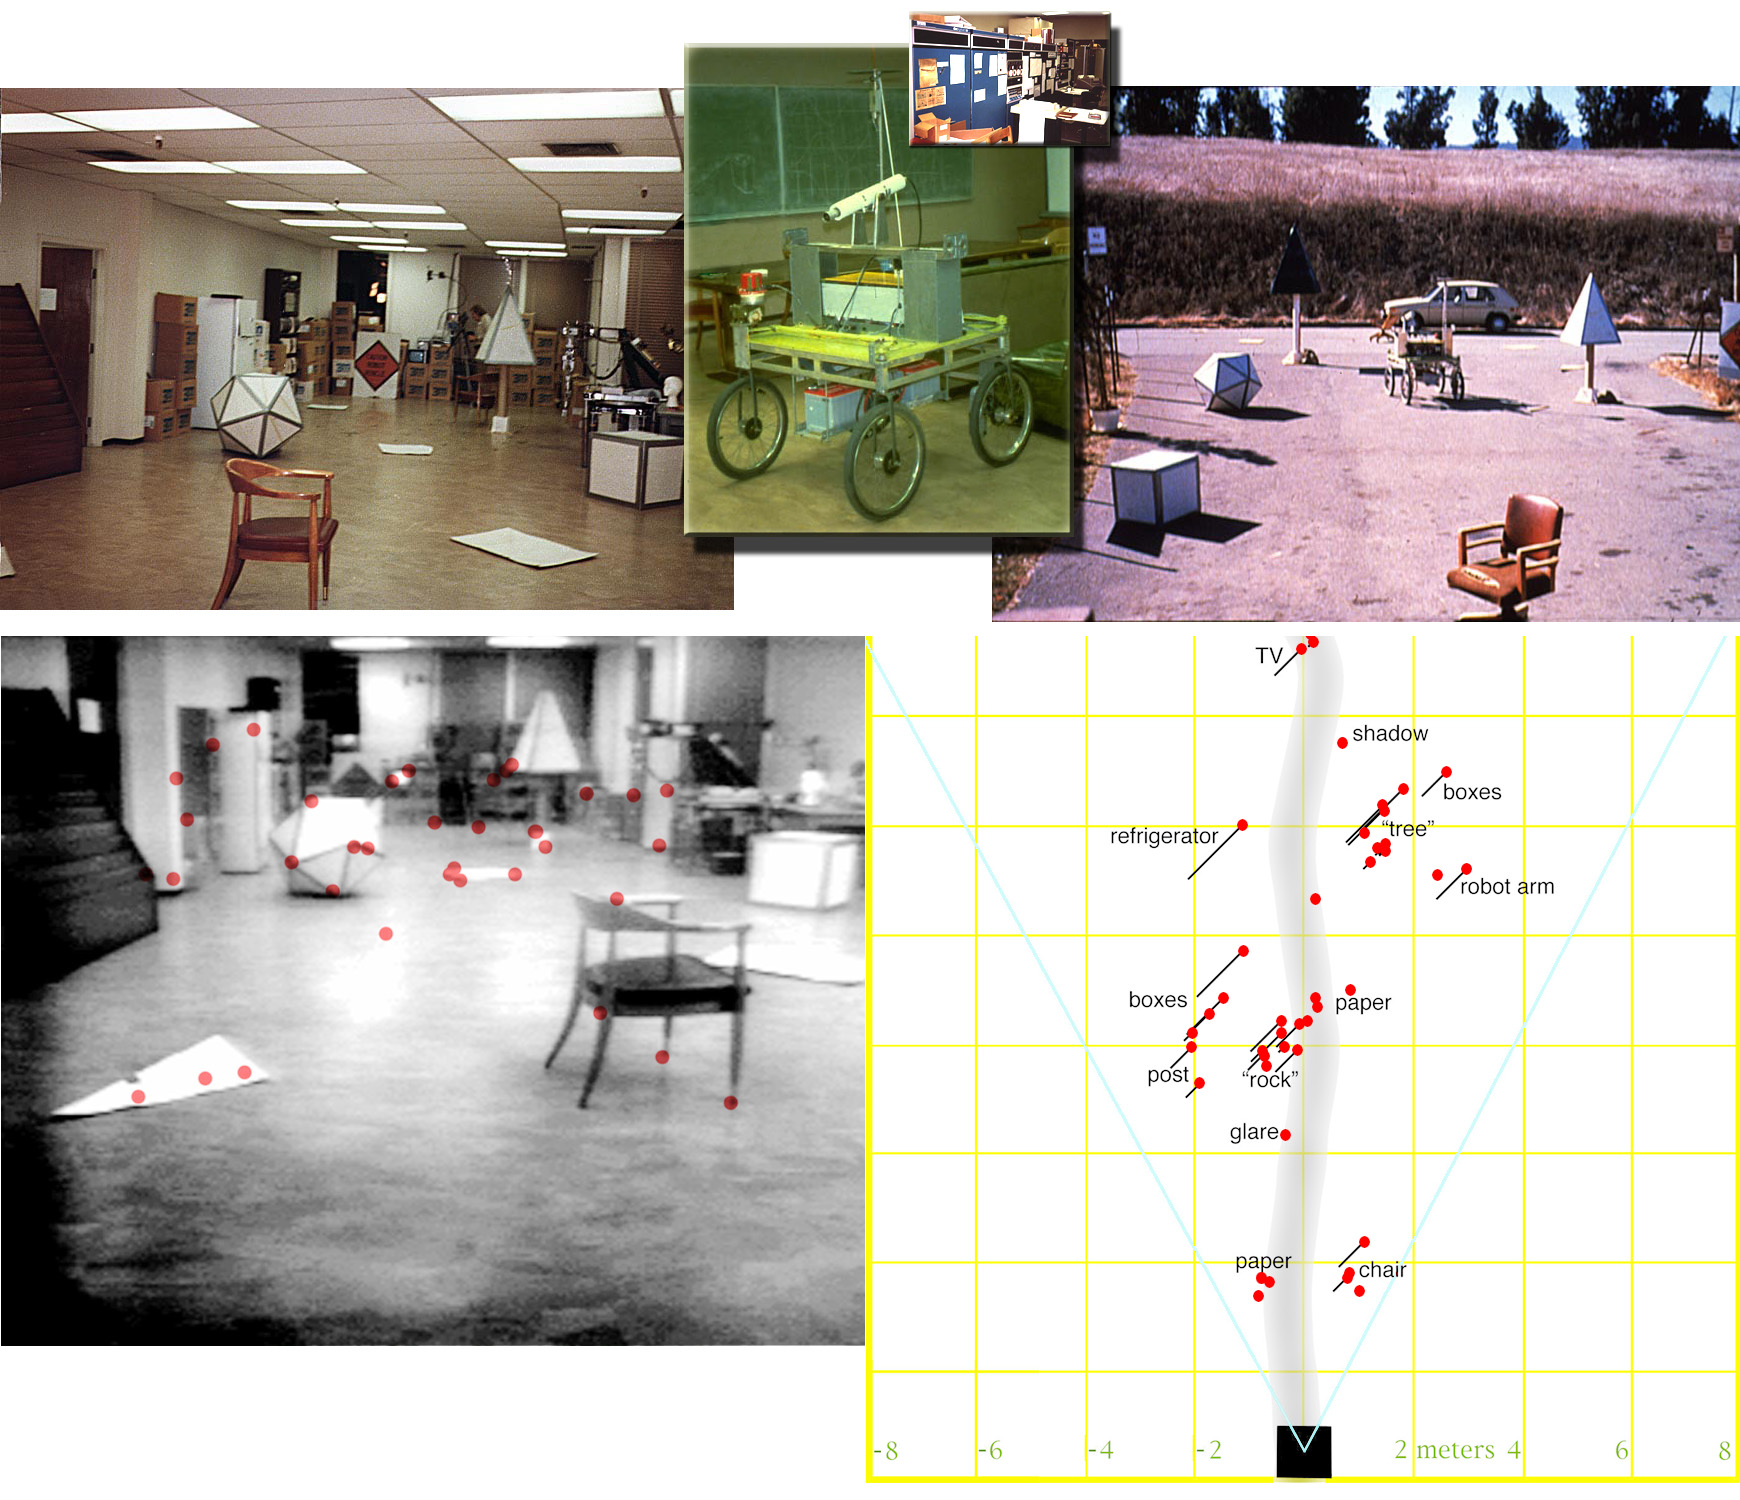
\includegraphics[width=\textwidth, clip, trim = 0 0 0 0]{TheStanfordCart/1979.MRL.image.jpg}
        \end{columns}
%*----------- notes
    \note[item]{Notes can help you to remember important information. Turn on the notes option.}
\end{frame}
%-
%*----------- SLIDE -------------------------------------------------------------
\begin{frame}[c]{Observações dos experimentos}
    \begin{columns}
        \column{.05\textwidth}
        \column{.45\textwidth}
        \begin{itemize} 
            \item Melhores resultados: Ambiente indoor
            \item Tempo de pausa: 10 a 15 minutos para processar as imagens e gerar a trajetória
            \item Deslocamento lento
            \item Bateria insuficiente para testes prolongados
            \item Tempo de execução do percurso: 5 horas
        \end{itemize}
        \column{.5\textwidth}
        \centering
            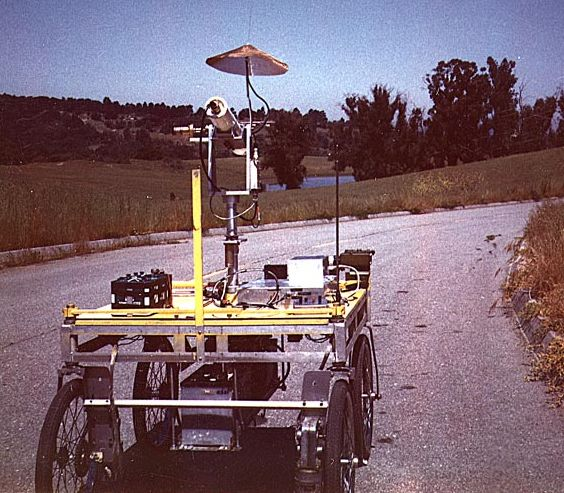
\includegraphics[width=0.8\textwidth, clip, trim = 0 0 0 0]{TheStanfordCart/StanfordCart-005.png}
        \end{columns}
%*----------- notes
    \note[item]{Notes can help you to remember important information. Turn on the notes option.}
\end{frame}

%*----------- SLIDE -------------------------------------------------------------
\begin{frame}[t]{The CMU Rover}
    \begin{columns}
        \column{.05\textwidth}
        \column{.45\textwidth}
            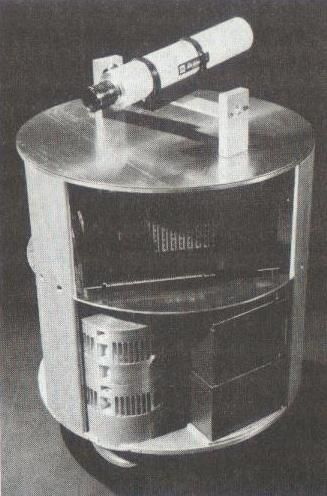
\includegraphics[width=0.6\textwidth, clip, trim = 0 0 0 0]{TheStanfordCart/CMU-Rover-Hollandp2-x640.jpg}
        \column{.5\textwidth}
            % \centering
           Comparação com o Stanford Cart
            \begin{itemize} 
                \item Possui um sistema mais sofisticado
                \item É mais rápido
                \item Possui um sistema mais flexível
            \end{itemize}
            \end{columns}
%*----------- notes
    \note[item]{Notes can help you to remember important information. Turn on the notes option.}
\end{frame}

%*----------- SLIDE -------------------------------------------------------------
\begin{frame}[c]{Características do CMU Rover}
    \begin{columns}
        \column{.05\textwidth}
        \column{.45\textwidth}
        \begin{itemize} 
            \item É cilíndrico
            \item Possui 3 GDL nas rodas
            \item Apresenta vários sensores
        \end{itemize}
        \column{.5\textwidth}
            \centering
                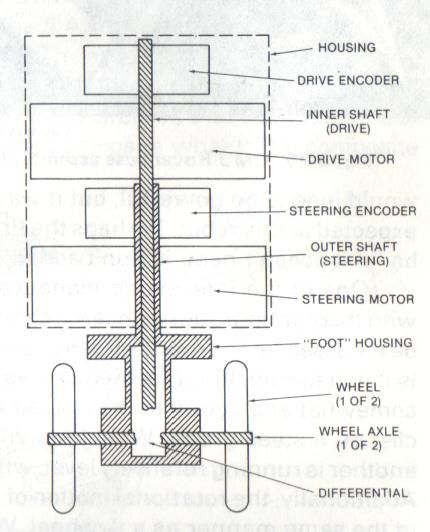
\includegraphics[width=0.75\textwidth, clip, trim = 0 0 0 0]{TheStanfordCart/CMU-Rover-Hollandp3-x640.jpg}
            \end{columns}
%*----------- notes
    \note[item]{Notes can help you to remember important information. Turn on the notes option.}
\end{frame}
%*----------- SLIDE ------------------------------------------------------------
\begin{frame}
    %\transdissolve[duration=0.5]
    %\hspace*{-1cm}
    \begin{columns}
        %\column{.01\textwidth}
        \column{0.30\textwidth}
        ~\hfill
            \begin{beamercolorbox}[sep=8em, colsep*=18pt, wd=\textwidth,ht=\paperheight]{title page header}
                \begin{center}
                    \textbf{\huge{Conclusão}}\par
                    % \vspace*{0.3cm}
                    % \textbf{\huge{LIBERDADE}}\par
                    \vspace*{0.3cm}
                    The Stanford Cart and The CMU Rover
                \end{center}
            \end{beamercolorbox}%         
        \column{.05\textwidth} 
        \column{.65\textwidth}
        \begin{center}
            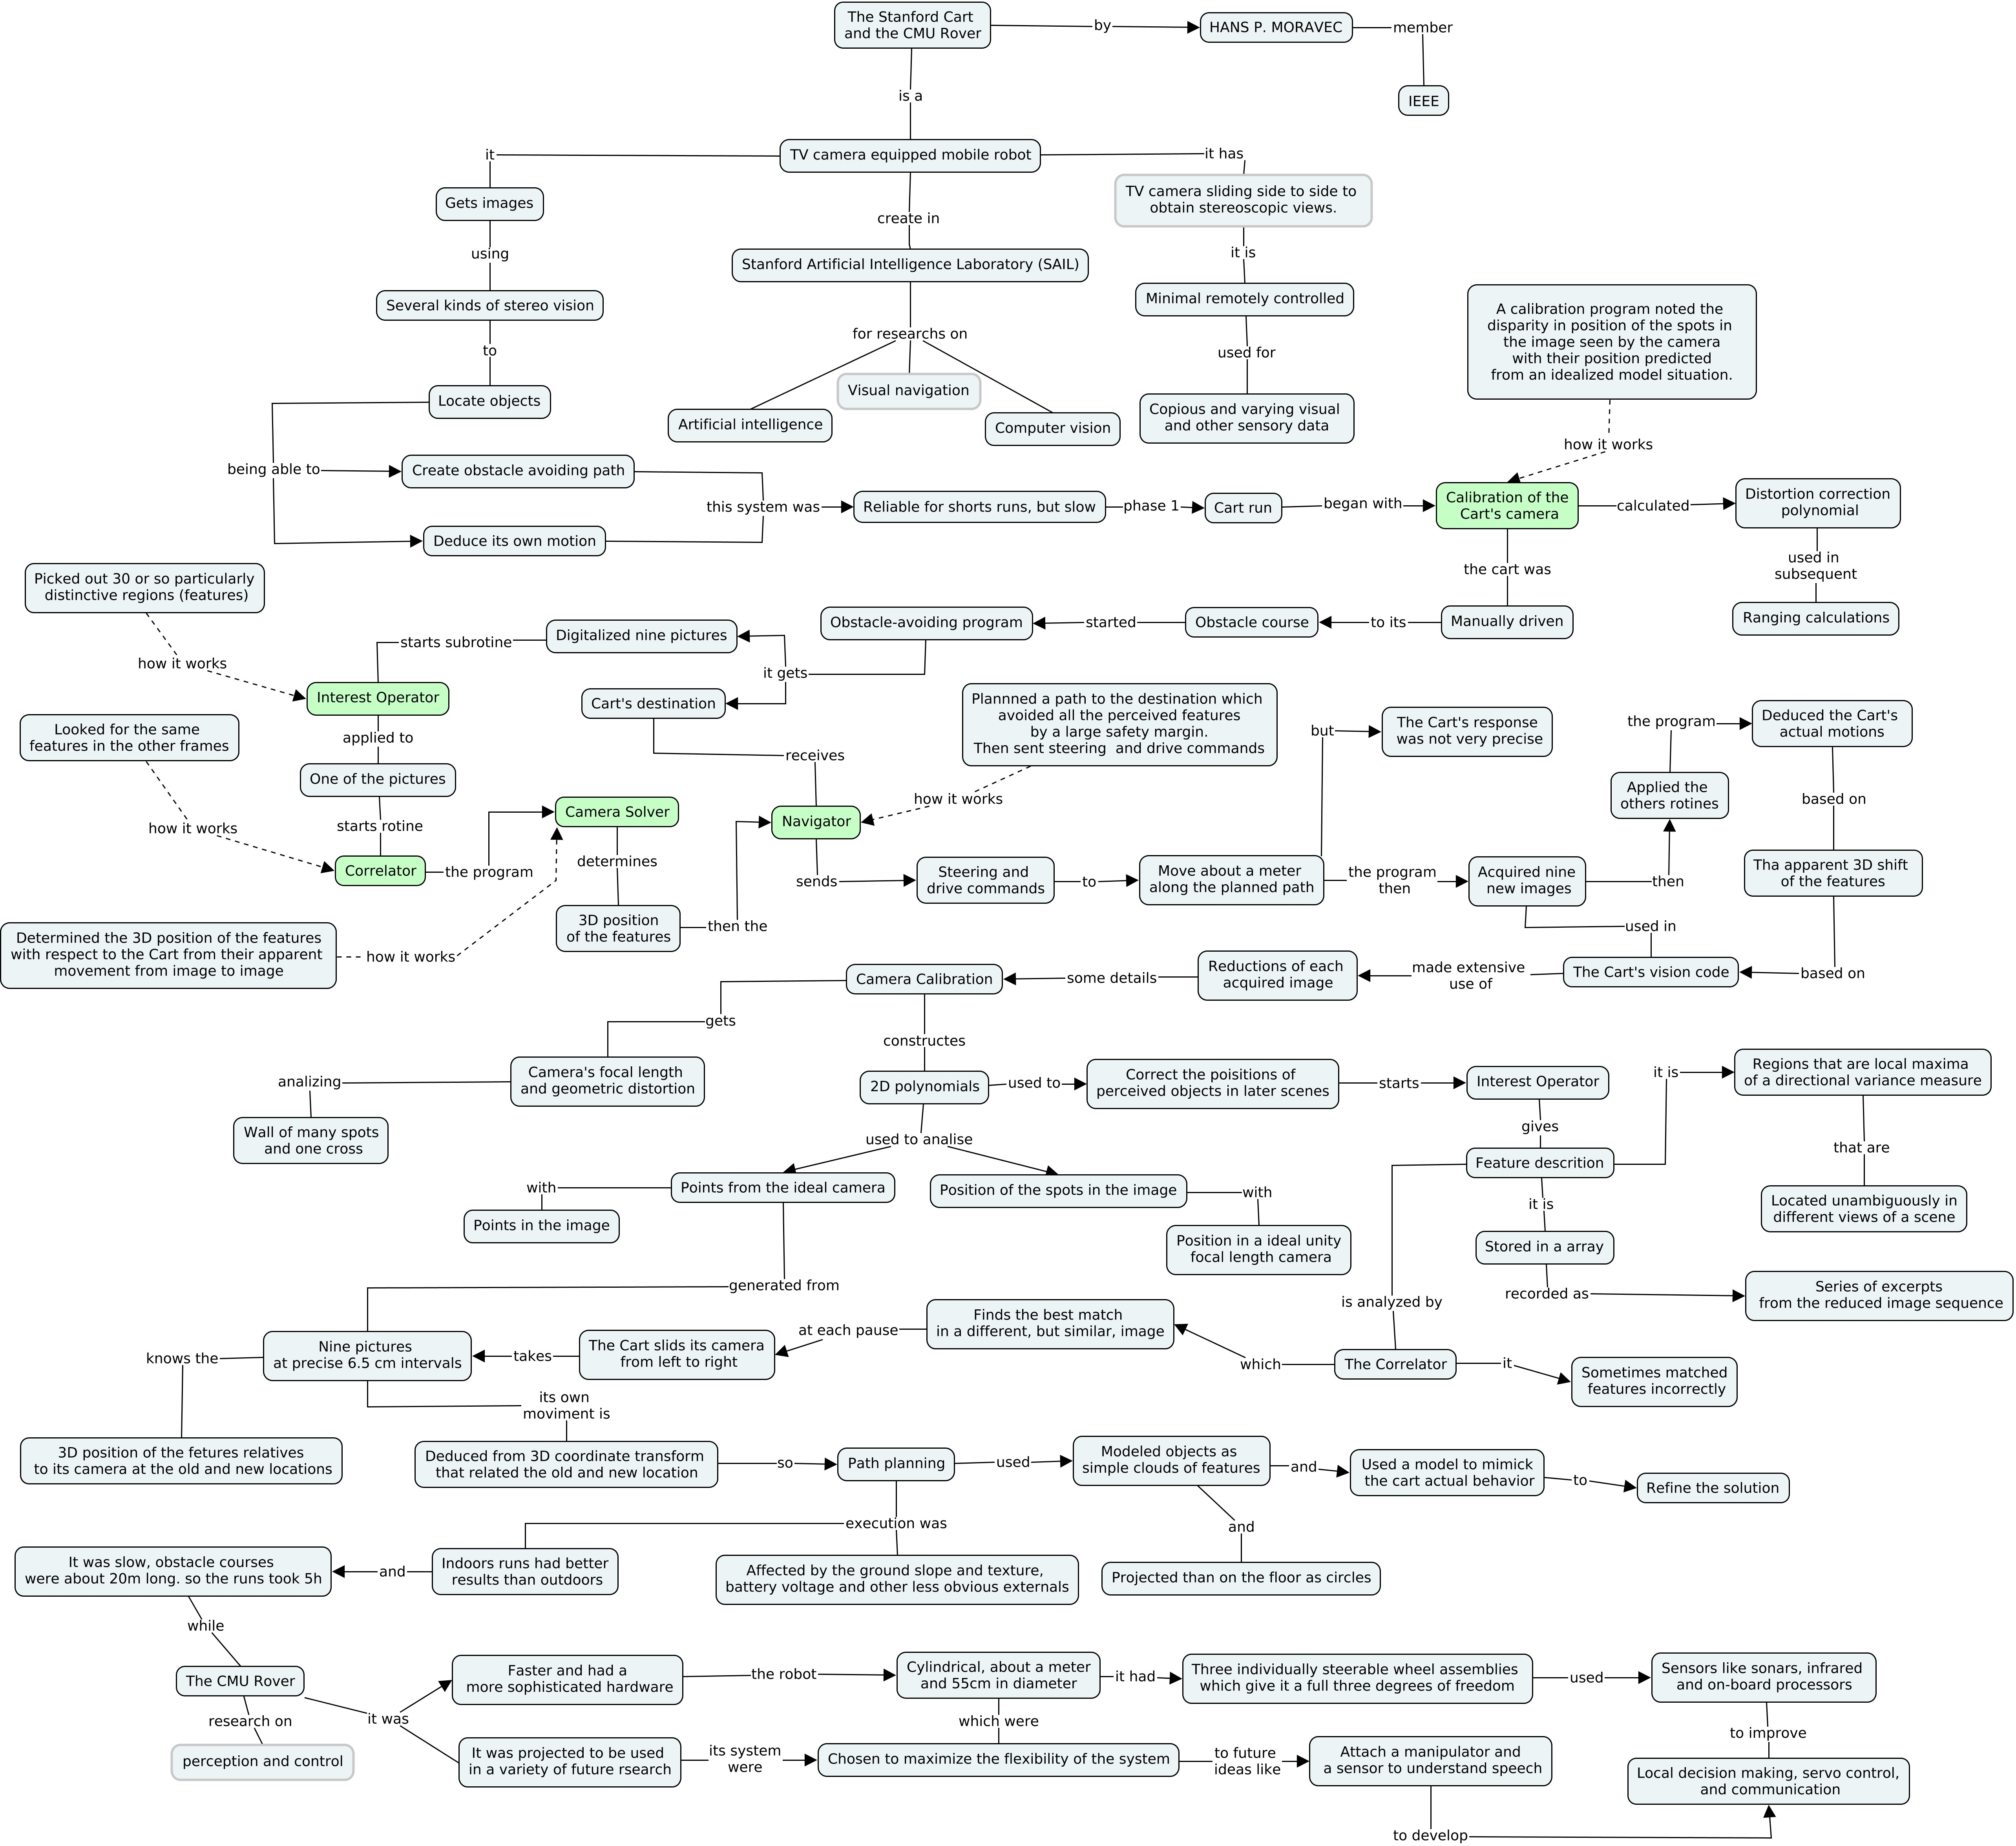
\includegraphics[width=0.85\textwidth]{TheStanfordCart/The Stanford Cart and The CMU Rover.jpg}
        \end{center}
            
    \end{columns}
  
%*----------- notes
    \note[item]{Notes can help you to remember important information. Turn on the notes option.}
 \end{frame}
%-